\documentclass[dvipsnames,10pt]{beamer}
\usepackage{ucltemplate}
\usepackage{tikz}
\usetikzlibrary{arrows,shapes, backgrounds, decorations.pathmorphing}
\usepackage{graphicx}
\usepackage{amssymb,amsmath}
\usepackage{listings}
\usepackage{multimedia}
\usepackage{empheq}
\usepackage{makecell}
\usepackage[many]{tcolorbox}
\usepackage[labelformat=empty]{caption,subfig}
%\usepackage[usenames]{color}
%\usetheme{Madrid}
%\mode<presentation>
\setbeamertemplate{navigation symbols}{}
\tikzstyle{na} = [baseline=-.5ex]

\tcbset{highlight math style={enhanced,
  colframe=red!60!black,colback=yellow!50!white,arc=4pt,boxrule=1pt,
  }}


\def\bx{\mathbf{x}}
\def\by{\mathbf{y}}

\renewcommand\theadalign{bc}
\renewcommand\theadfont{\bfseries}
\renewcommand\theadgape{\Gape[4pt]}
\renewcommand\cellgape{\Gape[4pt]}

% From https://tex.stackexchange.com/questions/60216/how-to-create-a-squiggle-arrow-with-some-text-on-it-in-tikz
\newcounter{sarrow}
\newcommand\xrsquigarrow[1]{%
\stepcounter{sarrow}%
\begin{tikzpicture}[decoration=snake]
\node (\thesarrow) {\strut#1};
\draw[->,decorate] (\thesarrow.south west) -- (\thesarrow.south east);
\end{tikzpicture}%
}

\title{Electrostatic simulations with Bempp and Exafmm - A black-box coupling approach}
%\author{\texorpdfstring{Timo Betcke\newline\url{t.betcke@ucl.ac.uk}}{Betcke}}

%\institute[University College London]{Department of Mathematics \\
%  University College London}
\date{}

\begin{document}
\lstset{language=Python}
\tikzstyle{every picture}+=[remember picture]
\begin{frame}
% \vspace*{-0.94cm}
% \hspace*{-1.02cm}
%\noindent\includegraphics[scale=0.4]{1824logo}

% \vspace{-3cm}
\vspace{1cm}

\titlepage
\vspace{-2cm}
\begin{columns}[T]
\begin{column}{.48\textwidth}
\begin{center}
    Timo Betcke \\
    \url{t.betcke@ucl.ac.uk}\\
    University College London
\end{center}
\begin{tcolorbox}
Joint with:\\ Tingyu Wang, Christopher Cooper, and Lorena Barba
\end{tcolorbox}
\end{column}%
\hfill%
\begin{column}{.48\textwidth}
\includegraphics[width=5cm]{../figs/ucl_campus}

\end{column}%
\end{columns}
\textit{Excalibur-SLE: Exascale HPC for System Level Engineering\\
EPSRC Grant: EP/V001531/1}

\end{frame}

\begin{frame}
    \frametitle{Poisson-Boltzmann for virus simulations}

    \vspace{.3cm}

    \begin{minipage}{5cm}
        Solve Poisson-Boltzmann equation
        \begin{align}
            \Delta\phi_1 &= \frac{1}{\epsilon_1}\sum_{k}q_k\delta(\mathbf{r}, \mathbf{r}_k)~\text{in }\Omega_1\nonumber\\
            (\Delta - \kappa^2)\phi_2 &= 0~\text{in }\Omega_2\nonumber
        \end{align}
        Interface conditions on $\Gamma$:
        \begin{align}
            \phi_1 &= \phi_2,\nonumber\\
            \epsilon_1\frac{\partial\phi_1}{\partial\mathbf{n}} &= \epsilon_2\frac{\partial\phi_2}{\partial \mathbf{n}}\nonumber
    \end{align}

    \end{minipage}
    \begin{minipage}{5cm}
        \includegraphics[width=4cm]{../figs/implicit_solvent.pdf}
    \end{minipage}
    Let $\phi_1 = \phi_{reac} + \phi_{coul}$ ($\phi_coul$ is potential generated from the point charges only). Then
    want to compute the solvation energy
    \begin{tcolorbox}
        $$
        \Delta G_{solv}^{polar} = \frac{1}{2}\sum_{k=1}^{N_q}q_k\phi_{reac}(\mathbf{r}_k)
        $$
    \end{tcolorbox}

\end{frame}

\begin{frame}
    \frametitle{Boundary Integral Formulation}

    Exterior field formulation\footnote{Lu et. al., Proc. Natl. Acad. Sci. USA 103 (51) (2006) 19314-19319}
    
\begin{align}
    &\begin{multlined}[t][0.48\textwidth] \frac{\phi_{2,\Gamma}}{2}\left(\frac{\epsilon_1}{\epsilon_2}+1\right) - \left(K_Y^\Gamma - \frac{\epsilon_1}{\epsilon_2}K_L^\Gamma\right)(\phi_{2,\Gamma}) \\
    + \left(V_Y^\Gamma - V_L^\Gamma\right)\left( \frac{\partial}{\partial \mathbf{n}} \phi_{2,\Gamma} \right) = \sum_{k=0}^{N_q}  \frac{q_k}{4\pi\epsilon_2|\mathbf{r}_{\Gamma} - \mathbf{r}_k|}
    \end{multlined} \nonumber \\
    &\begin{multlined}[t][0.48\textwidth] -\frac{\epsilon_1}{\epsilon_2}\left(W_Y^\Gamma - W_L^\Gamma\right)(\phi_{2,\Gamma}) +  \frac{1}{2}\frac{\phi_{2,\Gamma}}{\partial\mathbf{n}}\left(1+\frac{\epsilon_1}{\epsilon_2}\right) \\
    + \left(\frac{\epsilon_1}{\epsilon_2}K_Y^{\prime\Gamma} - K_L^{\prime\Gamma}\right)\left( \frac{\partial}{\partial \mathbf{n}} \phi_{2,\Gamma} \right) = \sum_{k=0}^{N_q}  \frac{\partial}{\partial\mathbf{n}_\mathbf{r}}\left(\frac{q_k}{4\pi\epsilon_2|\mathbf{r}_{\Gamma} - \mathbf{r}_k|}\right)\nonumber
    \end{multlined}
\end{align}

Also possible to derive interior field formulation (due to Juffur) or simple 
direct coupling from first line of Calder\`{o}n projector. 
Exterior formulation most favourable in terms of conditioning.

\end{frame}

\begin{frame}
    \frametitle{Zika virus}
    \begin{minipage}{6cm}
        \begin{itemize}
            \item Around 1.6m atoms
            \item Generated mesh has around 10m surface elements
        \end{itemize}
    \end{minipage}
    \begin{minipage}{4cm}
        \includegraphics[width=4cm]{../figs/6CO8_assembly.png}
    \end{minipage}

\begin{tcolorbox}
    Use Galerkin BEM code Bempp-cl accelerated with fast particle interactions through Exafmm-t
\end{tcolorbox}

Outline of rest of talk:
\begin{itemize}
    \item A short introduction to Bempp-cl and Exafmm-t
    \item Black-box coupling strategies for Galerkin BEM
    \item Practical issues and ongoing work
\end{itemize}

\end{frame}

\begin{frame}
    \frametitle{Bempp-cl}
    \begin{itemize}
        \item Successor of the Bempp boundary element library.
        \item Fully developed using Python with fast OpenCL kernels for computational routines.
        \item Galerkin discretisation of operators for Laplace, Helmholtz, and Maxwell problems.
        \item Compute kernels can be run on CPU or offloaded to GPU.
        \item Core routines optimised for fast dense assembly of opertors.
        \item Library provides coupling interfaces to Exafmm, can be easily adapted to other
            fast particle summation libraries.
    \end{itemize}
\end{frame}

\begin{frame}
    \frametitle{Characteristics of Bempp-cl}
    \vspace{-.1cm}
    \begin{center}
        \begin{tabular}{cc}
            \includegraphics[width=5cm]{../figs/bempp_cl_overview.png} & 
            \includegraphics[width=5cm]{../figs/bempp_single_vs_double.png} \\
            \begin{minipage}{5cm}
                \vspace{-4cm}
                \begin{itemize}
                    \item Top: Structure of Bempp-cl
                    \item Top-Right: AVX acceleration in Bempp-cl
                    \item Bottom-Right: Offloading of a domain potential operator
                \end{itemize}
            \end{minipage}&
            \includegraphics[width=5cm]{../figs/gpu_offloading.png} 
        \end{tabular}
    \end{center}
\end{frame}

\begin{frame}
    \frametitle{Exafmm-t: High-Performance KIFMM}
    \vspace{-.1cm}
    \begin{center}
        \begin{tabular}{cc}
            \begin{minipage}{5cm}
                \begin{itemize}
                    \item Kernel-Independent FMM library.
                    \item Written in C++, Provides Python Interface.
                    \item Highly efficient at higher accuracies.
                \end{itemize}
            \end{minipage} &
            \includegraphics[width=5cm]{../figs/fmm_sketch.pdf} \\
            \includegraphics[width=4cm]{../figs/near_far_decomposition.pdf} &
            \includegraphics[width=4cm]{../figs/multipole_expansion.pdf}
        \end{tabular}
    \end{center}

\end{frame}
    
\begin{frame}
    \frametitle{Coupling Bempp-cl and Exafmm-t}

Let $A$ be the matrix representation of a Galerkin discretised boundary integral operator.
Let $x$ be any vector. Reformulate $Ax$ as

$$
Ax = P_{test}^T(G - C)P_{dom}x + Sx
$$

\begin{itemize}
    \item $P_{test}$ and $P_{dom}$ highly sparse matrices that map function space coefficients to particle weights at quadrature points.    \item $G$ is black-box operator evaluating particle sums over weights across all quadrature points across all elements.
    \item $C$ is sparse matrix that contains the particle interactions between neighboring triangles.
    \item $S$ is sparse matrix containing all singular Galerkin integrals in adjacent elements.
\end{itemize}

\end{frame}

\begin{frame}
    \frametitle{The correction matrix}

    \begin{center}
        \includegraphics[width=10cm]{../figs/triangles.png}
    \end{center}

    Problem: Any FMM code also evaluates the near-field.
    Near-field can contain adjacent triangles (singular quadrature rules), and
    non-adjacent triangles (standard triangle Gauss rule).

    \vspace{.5cm}

    The sources and target points in the FMM are arising from the
    non-singular quadrature rule.

    \vspace{.5cm}

    Solution: After FMM evaluation subtract out the regular quadrature rule
    contribution from adjacent triangles and add in the correct singular quadrature
    rule contribution.

\end{frame}

\begin{frame}
    \frametitle{Number of FMM passes per Operator}

    \begin{tabular}{c|c|c|c|c}
        Operator & $V$ & $K$ & $K'$ & $W_Y$, $W_L$ \\
        \hline
        FMM Passes & 1 & 3 & 1 & 6, 3 
    \end{tabular}

    \vspace{.5cm}

    Example: Double-Layer Potential Operator

    \begin{align}
        [K\phi](\mathbf{x}) &= \int_{\Gamma}
        \partial_{\mathbf{n(\mathbf{y})}}g(\mathbf{x}, 
        \mathbf{y})\phi(\mathbf{y})ds(\mathbf{y})\nonumber \\
        &= -\sum_{j=1}^3\left[\nabla_{\mathbf{x}} 
        g(\mathbf{x}, \mathbf{y})\right]_j\mathbf{n}_j(\mathbf{y})
        \phi(\mathbf{y})ds(\mathbf{y})\nonumber
\end{align}

Require three FMM passes for the three different densities $\tilde{\phi}_j(\mathbf{y}):=\mathbf{n}_j(\mathbf{y})\phi(\mathbf{y})$, $j=1,\dots, 3$.

\vspace{.5cm}

The transmission operator for the exterior Poisson-Boltzmann formulation requires {\color{red} 19 FMM passes}.

\end{frame}

\begin{frame}
    \frametitle{Poisson-Boltzmann for a sphere}

    \begin{center}
        \begin{tabular}{cc}
            \includegraphics[width=5cm]{../figs/sphere_fmm.pdf} &
            \includegraphics[width=5cm]{../figs/sphere_memory.pdf} \\
            \begin{minipage}{5cm}
                \vspace{-3.5cm}
                \begin{itemize}
                    \item FMM Expansion Order 5
                    \item 6 regular quadrature points per element
                    \item \textbf{Right} Blue: Laplace, 
                        Yellow: Yukawa, Green: Singular Correction, Red: Other
                \end{itemize} 
            \end{minipage} &
            \includegraphics[width=5cm]{../figs/sphere_gmres_derivative.pdf}
        \end{tabular}
    \end{center}
\end{frame}

\begin{frame}
    \frametitle{Results for Zika Virus}

    \begin{center}
        \includegraphics[width=8cm]{../figs/6CO8_potential.png}
    \end{center}

    40 Core Compute node. Total time: 139.5 minutes, GMRES time: 80 minutes, 18 GMRES iterations, Max RAM use: 43GB, $\Delta G_{solv} = -116254.9 kcal/mol$. Diagonal preconditioner through inverse of mass matrix with mass lumping.

\end{frame}

\begin{frame}
    \frametitle{The next step: Scalable fast solver framework}

    \vspace{.1cm}
    Goal: Create a fast solver framework for fast parallel forward evaluation and
    approximate inversion of integral operators.

    \vspace{\baselineskip} 

    {\color{blue} All component libraries developed in Rust with Rayon (multithreading)
    and MPI (across nodes) for parallelization.}
    \vspace{\baselineskip}

    Development Status:
    \begin{itemize}
    \item {\color{blue} rusty-green-kernel} AVX accelerated direct evaluation
        of Laplace, Helmholtz Green's functions. {\color{green} Usuable}.
    \item {\color{blue} rusty-tree} Serial and parallel Octree implementations.
        Serial tree implemented. 
        Parallel tree early stages. {\color{yellow} Partially implemented}.
    \item {\color{blue} rusty-compression} Fast randomized compression routines
        for approximate low-rank matrices. {\color{yellow} Mostly finished.}
    \item {\color{blue} rusty-translation} Implementation of M2M, 
        M2L, L2L, P2M, L2P operators
        based on numerical field compressions (KIFMM, etc.)
        {\color{red} In planning}
    \item {\color{blue} rusty-fmm} Serial and parallel FMM loops 
        {\color{red} In planning}
    \item {\color{blue} rusty-inverse} Evaluation of approximate inverses 
        {\color{red} Not yet started}
    \end{itemize}

\end{frame}

\begin{frame}
    \frametitle{Summary}

    \begin{itemize}
        \item Generic, practically usuable and efficient black-box coupling of Galerkin
            BEM and Exafmm.
        \item All computational results shown today steered through interactive Jupyter
            notebooks.
        \item Python glue language between the codes. High productivity through Jupyter
            interface.
        \item For links to paper, reproducible data and codes see\\
            \url{https://github.com/barbagroup/bempp_exafmm_paper}
    \end{itemize}

    \vspace{1cm}

    \begin{tcolorbox}
        Work supported through Exalibur-SLE: Exascale HPC for System Level Engineering 
    \url{https://excalibur-sle.github.io/}
    \end{tcolorbox}

\end{frame}

\end{document}

\begin{frame}
\frametitle{Collaborators and Funding}
\begin{itemize}
    \item {\color{blue}UCL Colleagues and Students:} Simon Arridge, Matthew Scroggs (now Cambrige), Erik Burman, Antigoni Kleanthous, Xiaoshu Sun
    \item {\color{blue}External Collaborators:} Carlos Jerez-Hanckes (UAI Chile), Elwin Van 't Wout (PUC Chile), Wojciech Smigaj (Simpleware Ltd), Anthony Baran (Met Office), Dirk Praetorius (TU Vienna), Alexander Haberl (formerly TU Vienna), Alex Strohmaier (Leeds)
    \item {\color{blue} Funding:}
    \begin{small}\begin{itemize}
        \item BEM++ - A high performance boundary element library (EP/I030042/1)
        \item BEM++ - Stage 2 (EP/K03829X/1)
        \item Novel boundary element based solvers for light scattering from complex ice crystals (NE/N008111/1)
        \item Optimising patient specific treatment plans for ultrasound ablative therapies in the abdomen (Optimus) (EP/P012434/1)
        \item Reducing the threat to public safety: Improved metallic objecte characterisation (EP/R002274/1)
        \item New electromagnetic simulation tools for composite materials for small and medium enterprises (InnovaChile)
        \item Mathematical Analysis of Casimir Interactions (Leverhulme)
    \end{itemize}\end{small}
\end{itemize}
    
\end{frame}

\begin{frame}{Bemp in Action}

\begin{center}
    \includegraphics[width=11.5cm]{applications.png}
\end{center}

\end{frame}

\begin{frame}{A primer on boundary integral equations}
    \begin{minipage}{5cm}
    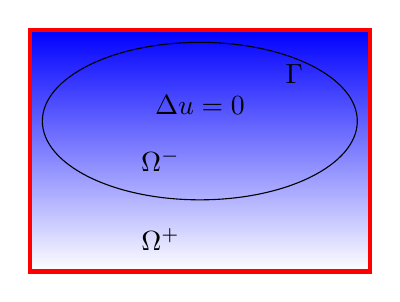
\begin{tikzpicture}[scale=1, framed,background rectangle/.style={ultra thick,draw=red, top color=blue}]
        \draw (0,0) ellipse (2cm and 1cm);
        \draw (.0,.2) node {$\Delta u = 0$};
        \draw (-.5, -.5) node {$\Omega^{-}$};
        \draw (1.2, .6) node {$\Gamma$};
        \draw (-.5, -1.5) node {$\Omega^{+}$};
    \end{tikzpicture}
\end{minipage}
\begin{minipage}{5cm}
Green's fct. for Laplace equation
$$
g(x, y) = \frac{1}{4\pi | x - y|}
$$
\end{minipage}

\vspace{.5cm}

{\color{red} Representation formula}
$$
u(x) = \int_{\Gamma}g(x, y)\tikz[baseline]{\node[fill=magenta!20, anchor=base] (t1) {$\gamma_1u(y)$};}ds(y) - \int_{\Gamma}\frac{\partial g(x, y)}{\partial n(y)}\tikz[baseline]{\node[fill=magenta!20, anchor=base] (t2) {$\gamma_0u(y)$};}ds(y),~x\in\Omega^{-}
$$
\tikz[na] \node[anchor=base] (n1) {Neumann trace}; \hspace{1cm} \tikz[na] \node[anchor=base] (n2) {Dirichlet trace};

\begin{tikzpicture}[overlay]
\path[->]<1-> (n1) edge [bend right] (t1);
\path[->]<1-> (n2) edge [bend right] (t2);
\end{tikzpicture}

\xrsquigarrow{Trace + Representation Formula}~ {\color{red}Calder\'{o}n identities}
\end{frame}

\begin{frame}{Calder\'{o}n identities}
\vspace{.5cm}
Take the Dirichlet and Neumann trace to obtain
\only<1>{
\begin{small}
\begin{empheq}[box=\tcbhighmath]{align}
    \gamma_0 u(x) &= \frac{1}{2}\gamma_0u(x) - \int_{\Gamma}\frac{\partial g(x, y)}{\partial n(y)} \gamma_0 u(y) ds(y) + \int_{\Gamma}g(x, y)\gamma_1 u(y) ds(y)\nonumber\\
    \gamma_1 u(x) &= \frac{1}{2}\gamma_1u(x)-\frac{\partial}{\partial n(x)}\int_{\Gamma}\frac{\partial g(x, y)}{\partial n(y)}\gamma_0u(y) ds(y) +\int_{\Gamma}\frac{\partial g(x, y)}{\partial n(x)}\gamma_1u(y) ds(y) \nonumber
\end{empheq}
\end{small}
}
\onslide<2->{
\begin{small}
\begin{empheq}[box=\tcbhighmath]{align}
    \gamma_0 u(x) &= \frac{1}{2}\gamma_0u(x) - [K\gamma_0u](x) + [V\gamma_1u](x)\nonumber\\
    \gamma_1 u(x) &= \frac{1}{2}\gamma_1u(x) + [W\gamma_0u](x) +[K'\gamma_0u](y)\nonumber
\end{empheq}
\end{small}
}
\onslide<3->{
\begin{center}
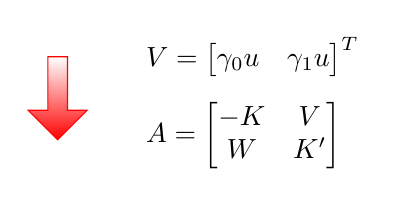
\begin{tikzpicture}
\draw (0, 0) node [single arrow, draw=red, top color=white, bottom color=red, minimum height=3em, outer sep=0pt,
       right=0pt, rotate=-90] {};
\draw (1, 0) node [anchor=west] {$V = \begin{bmatrix} \gamma_0u & \gamma_1u\end{bmatrix}^T$};
\draw (1, -1) node [anchor=west] {$A = \begin{bmatrix}-K & V\\ W & K'\end{bmatrix}$};
\end{tikzpicture}
\end{center}
\begin{columns}[T]
\begin{column}{.48\textwidth}
\begin{tcolorbox}
Interior Problem
$$
V = \left[\frac{1}{2}I + A\right]V
$$
\end{tcolorbox}
\end{column}
\begin{column}{.48\textwidth}
\begin{tcolorbox}
Exterior Problem
$$
V = \left[\frac{1}{2}I - A\right]V
$$
\end{tcolorbox}
\end{column}

\end{columns}
}

\end{frame}
\begin{frame}{Calder\'{o}n identities...}
\begin{itemize}
    \item Projection Property
    $$\left[\frac{1}{2}I \pm A\right]^2V = \left[\frac{1}{2}I \pm A\right]V$$
    for any possible pair of boundary data $V$.
    \item Regularisation Property
    $$
    \left(2A\right)^2 = I
    $$
\end{itemize}

\begin{block}{Outline}
\begin{itemize}
\item Efficient implementation of integral operators on modern CPU / GPU architectures
\item Benchmarks and Applications
\item Future developments
\end{itemize}
\end{block}
\end{frame}
\begin{frame}{How to discretise a boundary integral operator?}
Consider single-layer operator $V:H^{-1/2}(\Gamma)\rightarrow H^{1/2}(\Gamma)$
$$
[V\phi](x) = \int_{\Gamma}g(x, y)\phi(y)ds(y).
$$
Introduce (weak) variational form
$$
\langle V\phi, \psi\rangle_{\Gamma} = \int_{\Gamma}\psi(x)\int_{\Gamma}g(x, y)\phi(y)ds(y)ds(x),~\psi\in H^{-1/2}(\Gamma).
$$
\begin{columns}[T]
\begin{tcolorbox}[hbox]
\begin{column}{0.48\textwidth}
Compute matrix elements
$$
\mathbf{V}_{ij} = \int_{\tau_i}\int_{\tau_j} g(x, y)ds(y) ds(x)
$$
\end{column}
\end{tcolorbox}
 \begin{column}{0.48\textwidth}
 \vspace{-2.5cm}
 \begin{center}
\scalebox{.15}{\input{sphere.pgf}}
\end{center}
 \end{column}
 \end{columns}  
\end{frame}



\begin{frame}{Evaluating the kernel integrals}
\begin{columns}[T]
\begin{column}{.5\textwidth}
\textbf{Regular Integrals}

\vspace{\baselineskip}

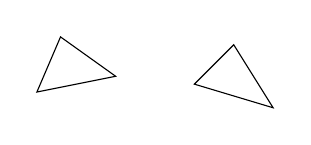
\begin{tikzpicture}
\draw  (0, 0) node {}
    -- (1, .2) node {}
    -- (.3, .7) node{}
    -- cycle;
\draw  (2, .1) node {}
    -- (3, -.2) node {}
    -- (2.5, .6) node {}
    -- cycle;
\end{tikzpicture}
\begin{itemize}
    \item Triangles separated
    \item Use standard symmetric triangle Gauss quadrature
\end{itemize}
\begin{tcolorbox}
Require fast evaluation of singular/regular integrals on modern CPU/GPU architectures.
\end{tcolorbox}

\end{column}
\begin{column}{.5\textwidth}
\textbf{Singular Integrals}

\vspace{\baselineskip}

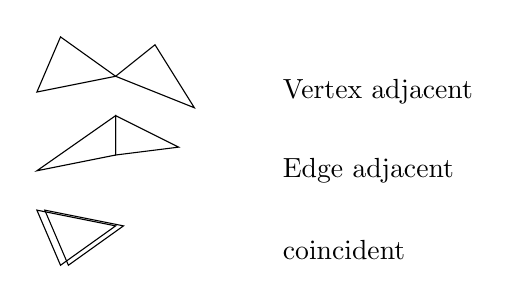
\begin{tikzpicture}
\draw  (0, 0) node {}
    -- (1, .2) node {}
    -- (.3, .7) node{}
    -- cycle;
\draw  (1, .2) node {}
    -- (2, -.2) node {}
    -- (1.5, .6) node {}
    -- cycle;
\draw  (0, -1) node {}
    -- (1, -.8) node {}
    -- (1, -.3) node{}
    -- cycle;
\draw (1, -.8) node {}
    -- (1, -.3) node {}
    -- (1.8, -.7) node {}
    -- cycle;
\draw  (0, -1.5) node {}
    -- (1, -1.7) node {}
    -- (.3, -2.2) node{}
    -- cycle;
\draw  (.1, -1.5) node {}
    -- (1.1, -1.7) node {}
    -- (.4, -2.2) node{}
    -- cycle;
\draw (3, 0) node[anchor=west] {Vertex adjacent};
\draw (3, -1) node[anchor=west] {Edge adjacent};
\draw (3, -2) node[anchor=west] {coincident};

\end{tikzpicture}
\begin{itemize}
    \item Need to distinguish adjacency of triangles
    \item We use fully numeric Erichsen/Sauter '98 rules
    %\item Can use analytical rules (e.g. Rjasanow/Steinbach '07) or expansion based methods (QBX, etc. Kl\"{o}ckner et. al. '12)
\end{itemize}


\end{column}
\end{columns}
\end{frame}

\begin{frame}{A very brief primer on OpenCL}
\begin{minipage}{5cm}
\begin{center}
    \includegraphics[width=5cm]{opencl_overview.png}
\end{center}
\end{minipage}
\begin{minipage}{5cm}
\begin{small}
\begin{itemize}
\item Heterogeneous compute model
\item MIMD/SIMD/SIMT support
\item C99 based kernel language
\item Current version 2.2
\item OpenCL drivers by Intel, AMD, Nvidia plus open-source
\end{itemize}
\end{small}
\end{minipage}
\begin{minipage}{5cm}
\begin{small}
\begin{itemize}
\item Each device consists of compute units (e.g. CPU cores) and processing elements (e.g. SIMD lanes)
\item Work items arranged into work groups
\item Memory synchronization only inside a workgroup
\item Excellent Python support through PyOpenCL by Andreas Kloeckner
\end{itemize}
\end{small}
\end{minipage}
\begin{minipage}{5cm}
\begin{center}
    \includegraphics[width=5cm]{cl_workgroups.png}
\end{center}
\end{minipage}


\end{frame}

\begin{frame}{Compute kernels for regular integrals}
\begin{itemize}
    \item We have developed computational kernels for CPU / GPU architectures.
    \item On GPUs each regular triangle pair is one independent work item (Launch $10^8$ work items for a matrix of dimension 10,000).
    \item On CPUs group work one test triangle with 4, 8, or 16 trial triangles to efficiently target SIMD lanes (either AVX2 or AVX-512, depending on CPU model).
    \item Adjacent triangles computed with regular kernels, but results discarded.
\end{itemize}
\end{frame}

\begin{frame}{Kernels for singular integrals}
\begin{itemize}
    \item Large number of quadrature points (typically well over 1k per triangle pair).
    \item Create workgroups of tasks for each triangle pair that split the kernel evaluations.
    \item All singular quadrature rules loaded together onto device. Each pair associated with pointer into corresponding rule (avoid if-branching)
    \item Result stored as sparse matrix or summed into final dense matrix.
\end{itemize}
\end{frame}

\begin{frame}{The Bempp-cl software}
\begin{columns}[T]
\begin{column}{.5\textwidth}
\begin{itemize}
    \item New development of the Bempp library for boundary element discretisations
    \item Written in Python + OpenCL kernels
    \item Over 30k lines of code
\end{itemize}
\end{column}
\begin{column}{.5\textwidth}
\vspace{-\baselineskip}
\begin{center}
    \includegraphics[width=5cm]{bempp_logo}
\end{center}
\end{column}
\end{columns}
Support for
\begin{itemize}
    \item Laplace, Helmholtz, modified Helmholtz single layer, double layer, adjoint double layer, hypersingular operators
    \item Maxwell electric and magnetic field integral operators
    \item Fast dense discretisation on Intel/AMD CPUs (using AVX2 or AVX-512); Nvidia, Intel, AMD GPus.
    \item Complete operator algebra.
    \item Flat structure. Small layer below the interface that calls into OpenCL compute kernels.
\end{itemize}

\end{frame}

\begin{frame}{Acceleration technologies}

\begin{minipage}{5cm}
\begin{small}
{\color{blue} Numba}
\begin{itemize}
    \item Grid topology computations
    \item Python callables
    \item Routines on functions, (integration, etc.)
\end{itemize}
\end{small}
\end{minipage}
\begin{minipage}{5cm}
\begin{small}
{\color{blue} OpenCL}
\begin{itemize}
    \item All potential evaluations
    \item Mass matrices
    \item FMM Near-Field
\end{itemize}
\end{small}
\end{minipage}

\vspace{\baselineskip}

\begin{small}
{\color{blue} Other technologies }
\begin{itemize}
    \item Python multiprocessing to drive multiple GPUs
    \item Scipy for spare matrix operations and iterative solvers
    \item Numpy dense solvers
    \item Dask for distributed FMM task management (early experiments)
\end{itemize}
\end{small}

\end{frame}

\begin{frame}{Example: Defining a grid function}
Given basis functions $\phi_j(x)$ and arbitrary function $f$. Want to approximate
$$
f(x) \approx \sum_{j=1}^Nc_j\phi_j(x),~x\in\Gamma.
$$
Use Galerkin projection with suitable dual basis $\psi_i(x)$ to obtain projection coefficients
$$
p_i(x) = \int_{\Gamma}f(x)\psi_i(x)ds(x).
$$
Solve linear system $Mc = p$ with $M_{ij} = \int_{\Gamma}\psi_i(x)\phi_j(x)ds(x)$.
    
\end{frame}

\begin{frame}{Implementation in Bempp-cl}
\begin{columns}[T]
\begin{column}{.5\textwidth}
\includegraphics[width=6cm]{grid_fun_definition.png}
\end{column}
\begin{column}{.5\textwidth}
\begin{itemize}
    \item Python is just-in-time compiled using Numba
    \item Projection coefficients computed in Numba accelerated loop
    \item Mass matrix setup with OpenCL
\end{itemize}
\end{column}
\end{columns}

\begin{tcolorbox}
Solve for coefficients only when needed (all Bempp evaluations are lazy)
\end{tcolorbox}

\end{frame}

\begin{frame}{Example: Defining a boundary operator}
\includegraphics[width=10cm]{operator_definition.png}

\begin{itemize}
    \item Operators take 3 space inputs (domain, range, and dual space)
    \item Depending on the underlying device, OpenCL code is compiled just-in-time and executed
    \item Actual matrix assembly first happens when required
\end{itemize}



\end{frame}

\begin{frame}{A first application}
\begin{tcolorbox}
Computing the capacity of polyhedra in three dimensions.
\end{tcolorbox}
Exterior Laplace problem
\begin{align}
    -\Delta u &= 0 \text{ in } \Omega^{+}\nonumber\\
            u &= 1   \text{ on } \Gamma\nonumber\\
            |u(x)| &= \mathcal{O}\left(|x|^{-1}\right) \text{ as } |x|\rightarrow\infty\nonumber
\end{align}
Normalised Capacity: $\text{cap}(\Omega) = -\frac{1}{4\pi}\int_{\Gamma}\frac{\partial u}{\partial \nu}(x)ds(x)$.

\vspace{\baselineskip}

{\color{red} Need to solve: } $V\frac{\partial u}{\partial \nu} = -1$.


\end{frame}

\begin{frame}{Single Layer Operator Assembly Timings}

\begin{center}
    \begin{tabular}{c|c|c|cc|cc|}
    \thead{N} & \thead{novec \\ single} & \thead{novec \\ double} & \thead{AVX2 \\ single} & \thead{AVX2 \\ double} & \thead{AVX-512 \\ single} & \thead{AVX-512 \\ double}\\
    \hline
    8192 & 1.6s  & 1.9s  & 0.7s  &  1.1s & 0.6s  &  1s\\
    32768 & 20.0s & 26.7s & 7.7s & 13.8s & 6.0s & 12.3s
    \end{tabular}
\end{center}

{\color{blue} Each kernel: } Perform all local geometry computations (faster than fetch from memory), evaluate Laplace kernel, sum into global matrix.

\vspace{\baselineskip}

AVX2: 4 / 8 (single/double precision) SIMD lanes\\
AVX-512: 8 / 16 (single/double precision) SIMD lanes

\vspace{\baselineskip} 10 Core Intel Xeon W-2155 3.3GHz base clock rate.

\end{frame}

\begin{frame}{Dense evaluation on GPUs}
\begin{itemize}
    \item GPUs memory restricted devices. Cannot store large matrices.
    \item Memory transfer slow. Do not want to transfer large amounts of data (for Laplace data transfer often slower than computation).
\end{itemize}

{\color{blue} \xrsquigarrow{Solution:}} Generate matrix elements on the GPU on-the-fly during a matvec. Only communicate results with main memory.

\begin{center}
    \includegraphics[width=5cm]{matvec_flow.png}
\end{center}

\end{frame}

\begin{frame}{GPU Experiment}
Use Azure Cloud Node with four Nvidia V100 GPUs.

Evaluate electric field integral operator on sphere with 130k elements (200k dofs).

\begin{center}
    \includegraphics[width=7cm]{host_device_assignment.png}
\end{center}

\begin{itemize}
    \item Require 6.6s per matvec
    \item Corresponds to around $6.1\times 10^{11}$ evaluations of Helmholtz Green's fct.
    \item Competitive timing to many FMM implementations at these dimensions (and no issues with
    matrix compression for oscillatory kernels). For large dimensions FMM eventually wins.
\end{itemize}
    
\end{frame}

\begin{frame}{A complex FEM/BEM coupling application}
Have bounded domain $\Omega\subset\mathbb{R}^{3}$. Solve
\begin{align}
    -\Delta u^{+}(x) - k^2 u^{+}(x) &=0,~x\in\mathbb{R}^3\backslash{\overline{\Omega}}\nonumber\\
    -\Delta u^{-}(x) - k^2n^2(x)u^{-}(x) &= 0,~x\in\Omega\nonumber,\\
    u^{-}(x) &= u^{+}(x),~x\in\Gamma\nonumber\\
    \frac{\partial u^{-}}{\partial n(x)} &= \frac{\partial u^{+}}{\partial n(x)},~x\in\Gamma\nonumber
\end{align}
with $u^{+} = u^{inc} + u^{s}$ in $\mathbb{R}^3\backslash{\overline{\Omega}}$; $u^{inc}$ is incident wave. $u^{s}$ satisfies Sommerfeld radiation conditions
$$
\lim_{|x|\rightarrow\infty}\left(\frac{\partial u^{s}}{\partial |x|} - iku^{s}\right) = 0.
$$
\begin{itemize}
    \item Use FEM for the interior problem and BEM for the exterior problem
    \item Schwarz-type impedance coupling for interior and exterior problem (see Bendali, Boubendir, Fares '07)
\end{itemize}

\end{frame}

\begin{frame}{Impedance coupling}
Define $p^{+} := \frac{\partial u^{+}}{\partial n}$, $p^{-} := \frac{\partial u^{-}}{\partial n}$

\vspace{\baselineskip}

Boundary conditions:
\begin{align}
    p^+ - \beta u^{+} &= \lambda^{+}\nonumber\\
    p^- + \beta u^{-} &= \lambda^{-}\nonumber
\end{align}
We couple the interior and exterior impedance data.
$$
\begin{array}{ccc}
    \lambda^{+} &:= &p^{-} - \beta u^{-}\\
    \lambda^{-} &:= &p^{+} + \beta u^{+}
\end{array}\Rightarrow
\begin{array}{ccc}
    \lambda^{+} &= \lambda^{-} - 2\beta u^{-}\\
    \lambda^{-} &= \lambda^{+} + 2\beta u^{+}
\end{array}
$$
Here, $\beta := -ik(1 + i\eta)$ with $\eta$ small damping parameter. With $2\beta u^{+} = T^{+}\lambda^{+} + f$, $-2\beta u^{-} = T^{-}\lambda^{-}$ have linear system
$$
\begin{bmatrix}
1 & -1 -T^{+}\\
-1 - T^{-} & 1
\end{bmatrix}
\begin{bmatrix}\lambda^{-} \\ \lambda^{+}\end{bmatrix} = 
\begin{bmatrix}b \\ 0\end{bmatrix}
$$
with $b$ describing the influence from the incident wave.

\end{frame}

\begin{frame}{Implementation remarks}
\begin{itemize}
    \item For exterior problem uses Bempp with stable impedance formulation
    \item Interior problem solved by FEniCS
    \item Bempp contains mapping operators between FeniCS domain and Bempp surface P1 spaces
    \item ... Notebook demonstration
    
\end{itemize}

\end{frame}

\begin{frame}{Final words...}

\begin{itemize}
    \item Have developed a high-performance CPU/GPU library using only Python + JIT Compilation + OpenCL.
    \item Easy deployment since no complication of complex C++ code.
    \item With reasonable effort created compute kernels that scale effectively on CPU and GPU architectures.
    \item Install from conda-forge via `conda install bempp-cl` (for Linux and Windows Subsystem for Linux)
\end{itemize}
    
\end{frame}


\end{document}


